%% Author_tex.tex
%% V1.0
%% 2012/13/12
%% developed by Techset
%%
%% This file describes the coding for rsproca.cls

\documentclass[]{rsos}%%%%where rsos is the template name


\usepackage[T1]{fontenc}
\usepackage[utf8]{inputenc}


% tightlist command for lists without linebreak
\providecommand{\tightlist}{%
  \setlength{\itemsep}{0pt}\setlength{\parskip}{0pt}}

% From pandoc table feature
\usepackage{longtable,booktabs,array}
\usepackage{calc} % for calculating minipage widths
% Correct order of tables after \paragraph or \subparagraph
\usepackage{etoolbox}
\makeatletter
\patchcmd\longtable{\par}{\if@noskipsec\mbox{}\fi\par}{}{}
\makeatother
% Allow footnotes in longtable head/foot
\IfFileExists{footnotehyper.sty}{\usepackage{footnotehyper}}{\usepackage{footnote}}
\makesavenoteenv{longtable}



%%%% *** Do not adjust lengths that control margins, column widths, etc. ***

%%%%%%%%%%% Defining Enunciations  %%%%%%%%%%%
\newtheorem{theorem}{\bf Theorem}[section]
\newtheorem{condition}{\bf Condition}[section]
\newtheorem{corollary}{\bf Corollary}[section]
%%%%%%%%%%%%%%%%%%%%%%%%%%%%%%%%%%%%%%%%%%%%%%%

\begin{document}


%%%% Article title to be placed here
\title{Supplementary Inforamtion}

\author{
Carmen Cabrera$^{1}$,
Francisco Rowe$^{1}$}

\address{
  $^{1}$Geographic Data Science Lab, Department of Geography and Planning, University of Liverpool, Liverpool, United Kingdom.\\
  $^{}$}
%%%% Subject entries to be placed here %%%%
\subject{
subject 1,
subject 2,
subject 3}

%%%% Keyword entries to be placed here %%%%
\keywords{
one,
two,
optional,
optional,
optional}

%%%% Insert corresponding author and its email address}
\corres{
  Carmen Cabrera\\
  e-mail: \href{mailto:C.Cabrera@liverpool.ac.uk}{\nolinkurl{C.Cabrera@liverpool.ac.uk}}
}

%%%% Abstract text to be placed here %%%%%%%%%%%%
\begin{abstract}
The abstract text goes here. The abstract text goes here. The abstract text goes here. The abstract text goes here. The abstract text goes here. The abstract text goes here. The abstract text goes here. The abstract text goes here.
\end{abstract}
%%%%%%%%%%%%%%%%%%%%%%%%%%%

\providecommand{\EndFirstPage}{%
}

\maketitle

The main document should include:

Title (no more than 150 characters)

Author names and affiliations, and ORCID iDs where available

Abstract (no more than 200 words). (This will be used in reviewer
invitation emails so please think about how to describe your work to
make it easy for a potential reviewer to determine whether they would be
suitable.)

All main manuscript text. Ensure that all figures, tables and any
relevant supplementary materials are mentioned within the text
References

Acknowledgements and funding statement (ensure that you have included
grant numbers and the names of any funding providers)

Tables with captions Figure captions with credits where relevant

\newpage

\section{Alternative data aggregation approaches for Facebook data}\label{alternative-data-aggregation-approaches-for-facebook-data}

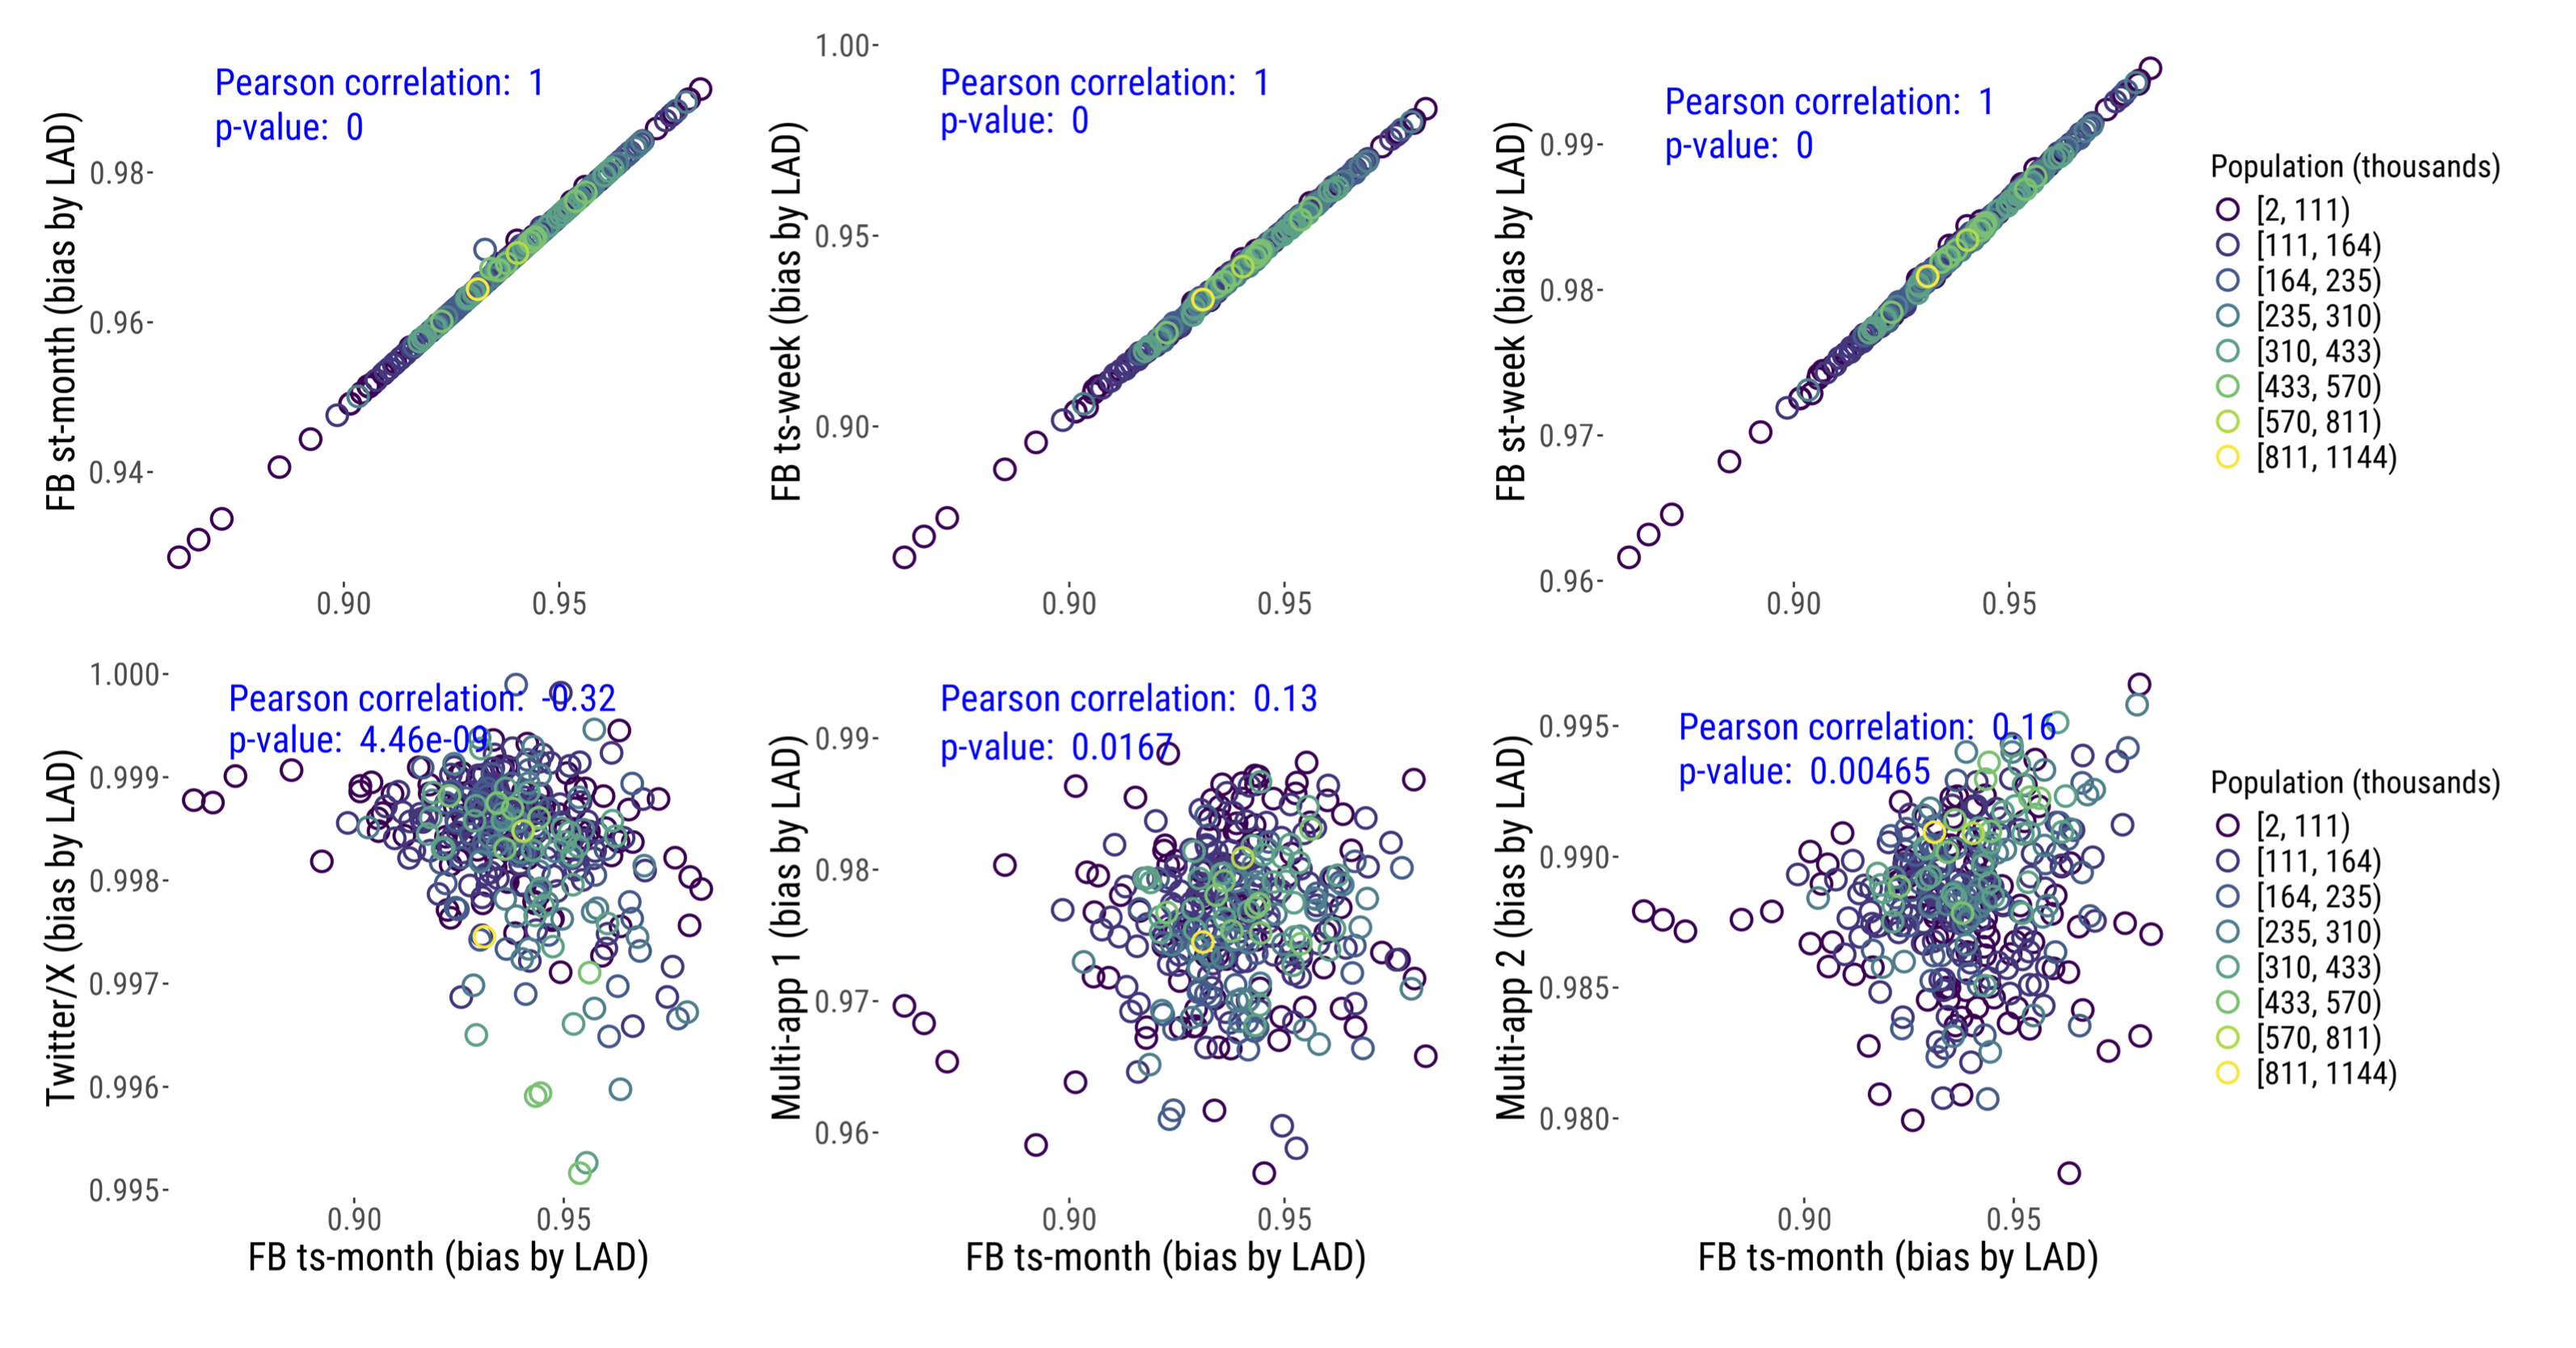
\includegraphics[width=5.35417in,height=2.58333in]{figures/Fig-compare-bias-size.png}

\section{Testing for spatial autocorrelation in the size of bias}\label{testing-for-spatial-autocorrelation-in-the-size-of-bias}

according to multiple spatial weighting schemes --\textgreater{} compute moran's I
and p-values, display them in a table (schemes as columns, data source
as rows)

\begin{figure}
\centering
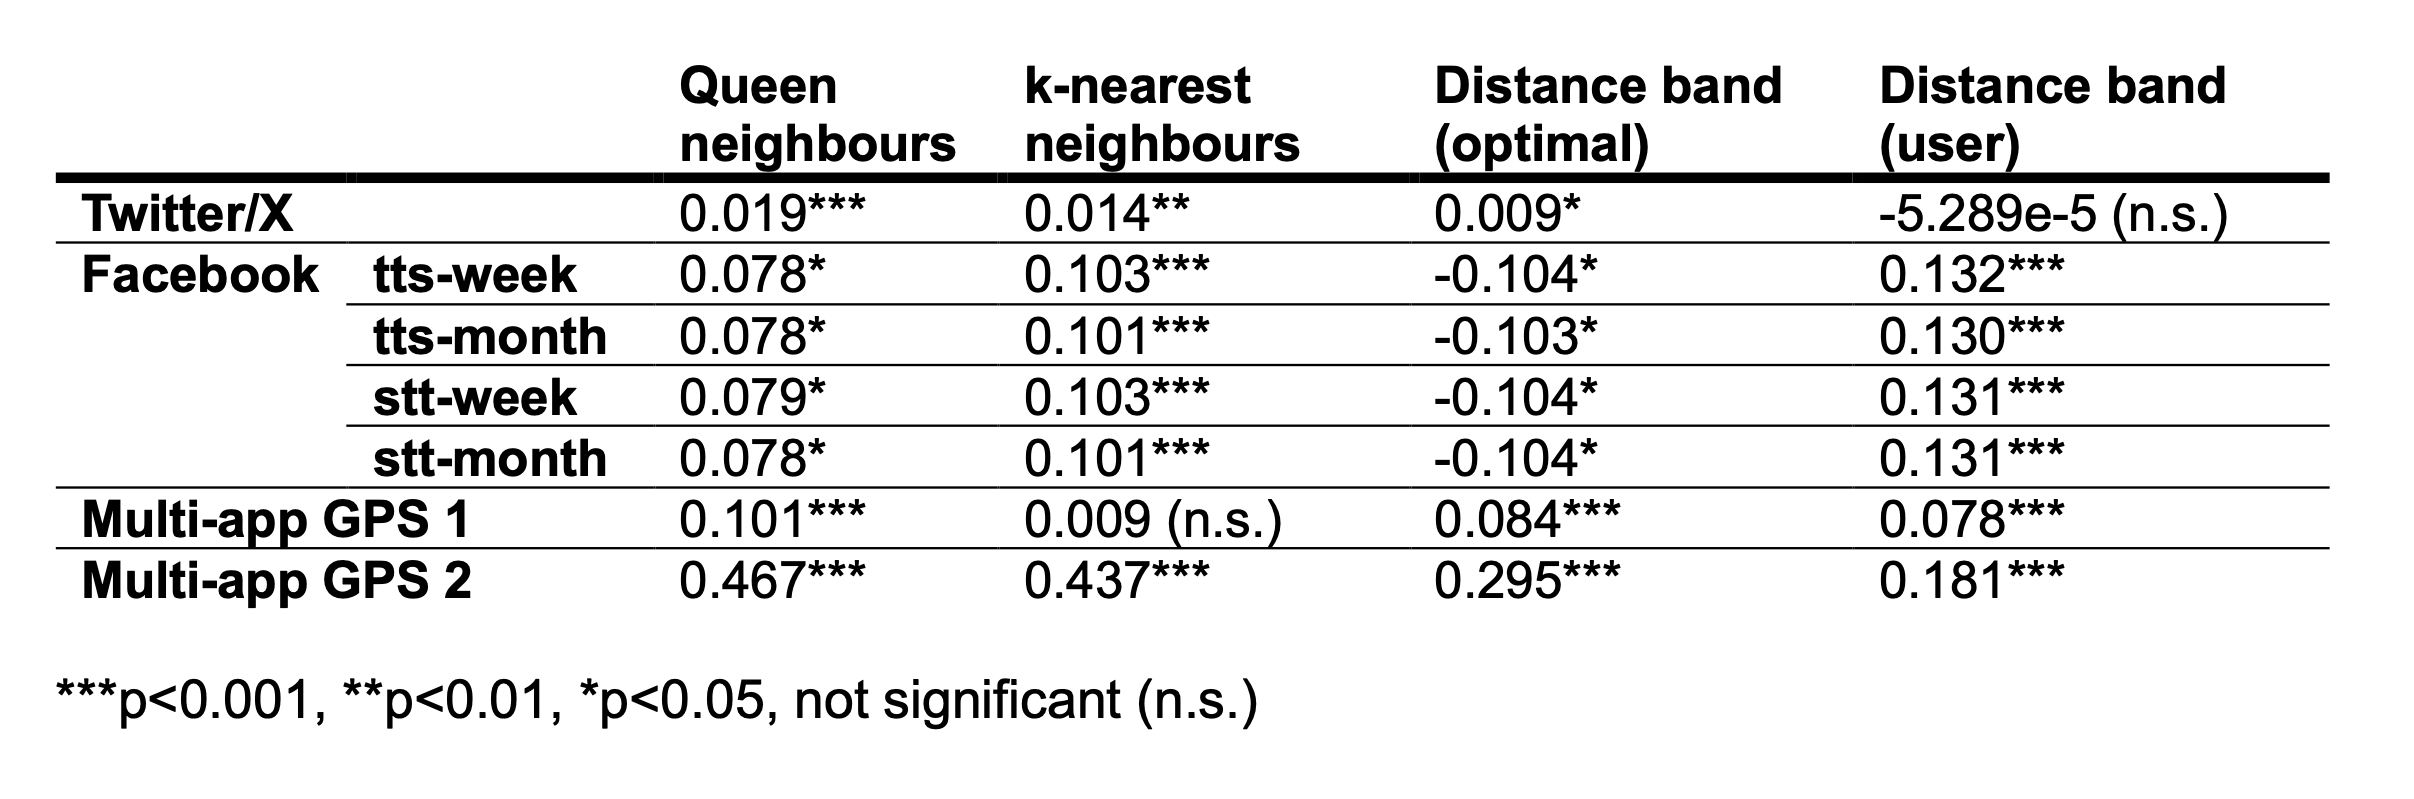
\includegraphics[width=5.20833in,height=2.29167in]{figures/Table-si.png}
\caption{Supplementary Table 1. Moran's I coefficients and significance,
computed according to four spatial weights schemes,}
\end{figure}

\ethics{Please provide details on the ethics.}

\dataccess{Please provide details on the data availability.}

\aucontribute{Please provide details of author contributions here.}

\competing{Please declare any conflict of interest here.}

\funding{Please provide details on funding}

\disclaimer{Please provide disclaimer text here.}

\ack{Please include your acknowledgments here, set in a single paragraph. Please do not include any acknowledgments in the Supporting Information, or anywhere else in the manuscript.}

\bibliographystyle{RS}
\bibliography{sample.bib}


\end{document}
